% Updated in February 2016 by Hwann-Tzong Chen
% Updated in May 2014 by Hideo Saito
% Updated in March 2012 by Yasuyuki Matsushita
% Updated in April 2002 by Antje Endemann, ...., and in March 2010 by Reinhard Klette
% Based on CVPR 07 and LNCS style, with modifications by DAF, AZ and elle 2008, AA 2010, ACCV 2010

\documentclass[runningheads]{llncs}
\usepackage{graphicx}
\usepackage{amsmath,amssymb} % define this before the line numbering.
\usepackage{ruler}
\usepackage{color}

%===========================================================
\begin{document}
\pagestyle{headings}
\mainmatter

\def\ACCVSubNumber{802}  % Insert your submission number here
\def\ACCV20SubNumber{\ACCVSubNumber}  % Compatibility with the ACCV ruler style.

%===========================================================
\title{TriPoseFusion: Robust Multi-View 3D Driver Pose Fusion with Outlier-Aware Canonicalization}
\titlerunning{ACCV submission ID \ACCVSubNumber}
\authorrunning{ACCV submission ID \ACCVSubNumber}

\author{Anonymous ACCV Submission}
\institute{Paper ID \ACCVSubNumber}

\maketitle

%===========================================================
\begin{abstract}
Robust 3D human pose estimation is a key component of driver monitoring and in-cabin behavior understanding, where reliable body geometry is needed under severe occlusion, limited camera placement, changing illumination, and fast hand or head motion. Although modern monocular pose estimators provide convenient per-view 3D keypoints, their predictions often contain viewpoint-dependent depth errors, missing joints, and temporal jitter. Multi-view cameras offer complementary observations, but directly averaging noisy monocular outputs is unreliable because per-view 3D predictions may live in inconsistent body frames. We propose \emph{TriPoseFusion}, a geometry-guided tri-view keypoint fusion framework centered on outlier-aware body canonicalization. The method first maps synchronized front/left/right predictions into a robust body-centered coordinate frame, then applies lightweight cross-view attention, joint-wise view gating, and temporal residual refinement to the normalized keypoint streams. TriPoseFusion is trained with self-supervised geometry objectives based on canonicalized pseudo teachers, view consistency, bone-length regularization, temporal smoothness, contrastive view alignment, and gate entropy regularization. Evaluation on 88 subject-environment sequences shows that TriPoseFusion reduces MPJPE from 2.078 m for the best single-view baseline to 0.412 m and improves PA-MPJPE from 1.275 m to 0.275 m against a corrected triangulation reference. Ablations show that robust canonicalization is the dominant source of this improvement, while the lightweight fusion and temporal modules provide a practical framework for operating on noisy synchronized keypoint streams. These results support robust geometry normalization as a simple but effective foundation for keypoint-level multi-view driver pose fusion.
\end{abstract}

%===========================================================
\section{Introduction}

Driver monitoring and in-cabin human understanding require stable 3D body pose representations. Fine-grained pose cues can support attention estimation, hand-state analysis, gesture understanding, safety intervention, and higher-level behavior recognition \cite{abouelnaga2017real,zhang2018driver,gorelik2026multiview}. Compared with ordinary human pose estimation in open scenes, the in-cabin setting is highly constrained: the driver is seated, cameras are mounted at fixed positions, and many safety-critical motions occur in a small upper-body workspace. These constraints provide useful structure, but they also create persistent visual challenges. The steering wheel, dashboard, seat, and arms often occlude hands and torso landmarks; camera viewpoints are limited by the vehicle layout; and illumination can change sharply between day, night, and low-light scenarios.

Monocular 3D pose estimators are attractive for this problem because they can be deployed independently on each camera stream and do not require a complete multi-view reconstruction pipeline \cite{toshev2014deeppose,martinez2017simple,mehta2017vnect}. However, monocular predictions are inherently ambiguous under depth uncertainty and become fragile when the visible evidence is partial. In driver monitoring, these limitations are especially pronounced for hands, wrists, shoulders, and head landmarks, which are repeatedly affected by steering-wheel occlusion, self-occlusion, motion blur, and detector noise. The resulting 3D keypoints may contain missing joints, inconsistent scale, incorrect depth ordering, and high-frequency jitter. Such errors are problematic not only for pose visualization, but also for downstream temporal reasoning, where noisy keypoints can be misinterpreted as meaningful driver motion.

Multi-view camera systems can alleviate these issues by observing the driver from complementary viewpoints \cite{iskakov2019learnable,qiu2019cross,tu2020voxelpose}. A joint invisible in the front camera may still be visible from a side camera, and depth ambiguity in one view can often be reduced by another. Nevertheless, practical multi-view fusion is not a simple averaging problem. First, different monocular estimators may produce keypoints in slightly different coordinate frames or with different scale and orientation biases. Second, view reliability is time-varying and joint-dependent: one camera may be reliable for the head and shoulders but unreliable for the hands, while another may provide the opposite pattern. Third, a corrupted view can be systematically wrong, so a fixed camera preference is insufficient. These observations suggest that robust fusion should reason about geometry, temporal motion, and per-joint view reliability jointly.

This paper studies the practical setting where synchronized front, left, and right cameras are available, but the fusion module receives only per-view keypoint outputs from an off-the-shelf monocular pose estimator. We propose \emph{TriPoseFusion}, a geometry-normalized tri-view 3D pose fusion framework for this noisy keypoint-to-keypoint setting. Rather than re-estimating pose from RGB images or relying on calibrated triangulation alone, TriPoseFusion learns to combine existing monocular 3D keypoint streams. The method first applies outlier-aware canonicalization to each view in a body-centered coordinate frame using upper-body geometry, reducing translation, orientation, and shoulder-baseline mismatch across views. It then constructs motion-aware per-joint features from 3D positions, multi-scale velocities, acceleration, and jerk. Cross-view attention allows the front/left/right tokens for the same joint and frame to exchange complementary evidence, while a joint-wise gating module provides a lightweight learned fusion interface. Finally, a dilated temporal convolutional refiner improves sequence-level stability by modeling longer-range motion context.

The proposed design is motivated by two principles. First, geometry normalization should be robust to unstable body landmarks, because small shoulder or neck errors can induce large coordinate-frame mismatch across monocular 3D predictions. Second, view-aware fusion and temporal refinement should operate after this robust alignment, because smoothing or weighting poorly aligned streams can preserve systematic view-specific artifacts. TriPoseFusion therefore combines outlier-aware geometry normalization, cross-view comparison, adaptive gating, and temporal residual correction in a unified framework. Since accurate 3D annotations are difficult to obtain in real vehicles, the model is trained with self-supervised geometry losses based on pseudo-teacher alignment, view consistency, bone-length constraints, temporal smoothness, contrastive view alignment, and gate entropy regularization \cite{rhodin2018learning,kocabas2019self,wandt2021canonpose}.

Our contributions are summarized as follows. First, we formulate robust driver pose recovery as noisy tri-view 3D keypoint fusion, focusing on the intermediate but practical representation between monocular pose estimation and downstream behavior recognition. Second, we introduce an outlier-aware body-centered canonicalization module that reduces cross-view coordinate-frame and shoulder-baseline mismatch before fusion and is the dominant contributor in our ablation. Third, we integrate this canonical representation with lightweight cross-view attention, joint-wise view gating, and temporal residual refinement, treating these modules as compact extensions around the core geometry normalization step. Fourth, we design a self-supervised training objective that uses pseudo-teacher alignment, multi-view consistency, motion smoothness, bone regularization, contrastive view alignment, and gate entropy to learn without manual 3D ground-truth annotation. Finally, we evaluate the method on 88 matched subject-environment sequences across day/night and high/low illumination settings using a corrected triangulation reference.

%-------------------------------------------------------------------------
\section{Related Work}
\label{sec:related}

\subsection{Monocular and Video-Based 3D Pose Estimation}
Monocular 3D pose methods recover joints by direct image-to-pose regression, 2D-to-3D lifting, or body-model regression \cite{toshev2014deeppose,martinez2017simple,zhou2017towards,mehta2017vnect,kanazawa2018end}. Video models further use temporal context to reduce frame-wise ambiguity and jitter \cite{pavllo20193d,kocabas2020vibe}. These approaches are useful for driver monitoring, but single-view recovery remains ill-posed under steering-wheel occlusion, viewpoint bias, truncation, and illumination changes. TriPoseFusion therefore treats monocular 3D keypoints as noisy observations and focuses on synchronously combining views rather than designing another monocular estimator.

\subsection{Multi-View Pose Estimation and Keypoint Fusion}
Multi-view methods improve observability through calibrated triangulation, semantic feedback, or by fusing image features, heatmaps, epipolar cues, and volumetric representations across cameras \cite{iskakov2019learnable,qiu2019cross,he2020epipolar,tu2020voxelpose,bultmann2021real,nogueira2024markerless}. Our setting is different: the fusion stage receives only per-view pose outputs from an existing monocular estimator, not raw images or dense heatmaps. This keypoint-level interface is lightweight and deployable, but it exposes the model to inconsistent 3D coordinate frames, missing joints, and view-dependent reliability. Fixed mean or median fusion assumes reliability is globally stable; TriPoseFusion instead learns joint-wise, time-varying reliability after robust body-centered alignment.

\subsection{Self-Supervised and Geometry-Guided Pose Learning}
Accurate 3D pose labels are difficult to obtain in real vehicles, so self-supervised methods and datasets use signals such as reprojection consistency, multi-view agreement, bone-length constraints, temporal smoothness, and triangulation-based pseudo labels \cite{rhodin2018learning,kocabas2019self,iskakov2019learnable,wandt2021canonpose,fan2023humanm3}. These signals can be brittle when a pseudo teacher contains outliers or one camera is corrupted. TriPoseFusion combines pseudo-teacher alignment, view consistency, bone regularization, temporal smoothness, contrastive view alignment, and gate entropy, targeting the practical gap between monocular keypoint extraction and full image-based multi-view reconstruction.

%===========================================================
\section{Method}
\label{sec:method}

\subsection{Problem Formulation}
Given $V=3$ synchronized views (front/left/right), the input to TriPoseFusion is
\begin{equation}
\left\{P_{v}^{3D}\right\}_{v=1}^{V},
\end{equation}
where $P_{v}^{3D}\in\mathbb{R}^{T\times J\times 3}$ denotes noisy monocular 3D keypoints for view $v$. The output is a fused 3D pose sequence
\begin{equation}
P_{\mathrm{final}}\in\mathbb{R}^{T\times J\times 3}.
\end{equation}
The goal is to recover a temporally stable and geometrically plausible pose from noisy multi-view keypoint estimates.

\subsection{Network Overview}
TriPoseFusion is implemented as a keypoint-to-keypoint fusion network rather than an image backbone or action classifier. Figure~\ref{fig:pipeline} summarizes the complete inference pipeline from synchronized in-cabin views to fused 3D keypoints. First, an off-the-shelf monocular pose estimator produces front, left, and right keypoint streams. The streams are organized as synchronized temporal sequences and canonicalized into an outlier-aware body-centered 3D coordinate frame. TriPoseFusion then constructs per-view motion-aware features from the canonicalized sequence, maps them with a shared view encoder, applies cross-view attention for view-aware interaction, and predicts joint-wise adaptive view weights. The resulting fused pose is passed through a dilated temporal refiner that predicts a residual correction and outputs the final fused 3D keypoints.

\begin{figure}[t]
\centering
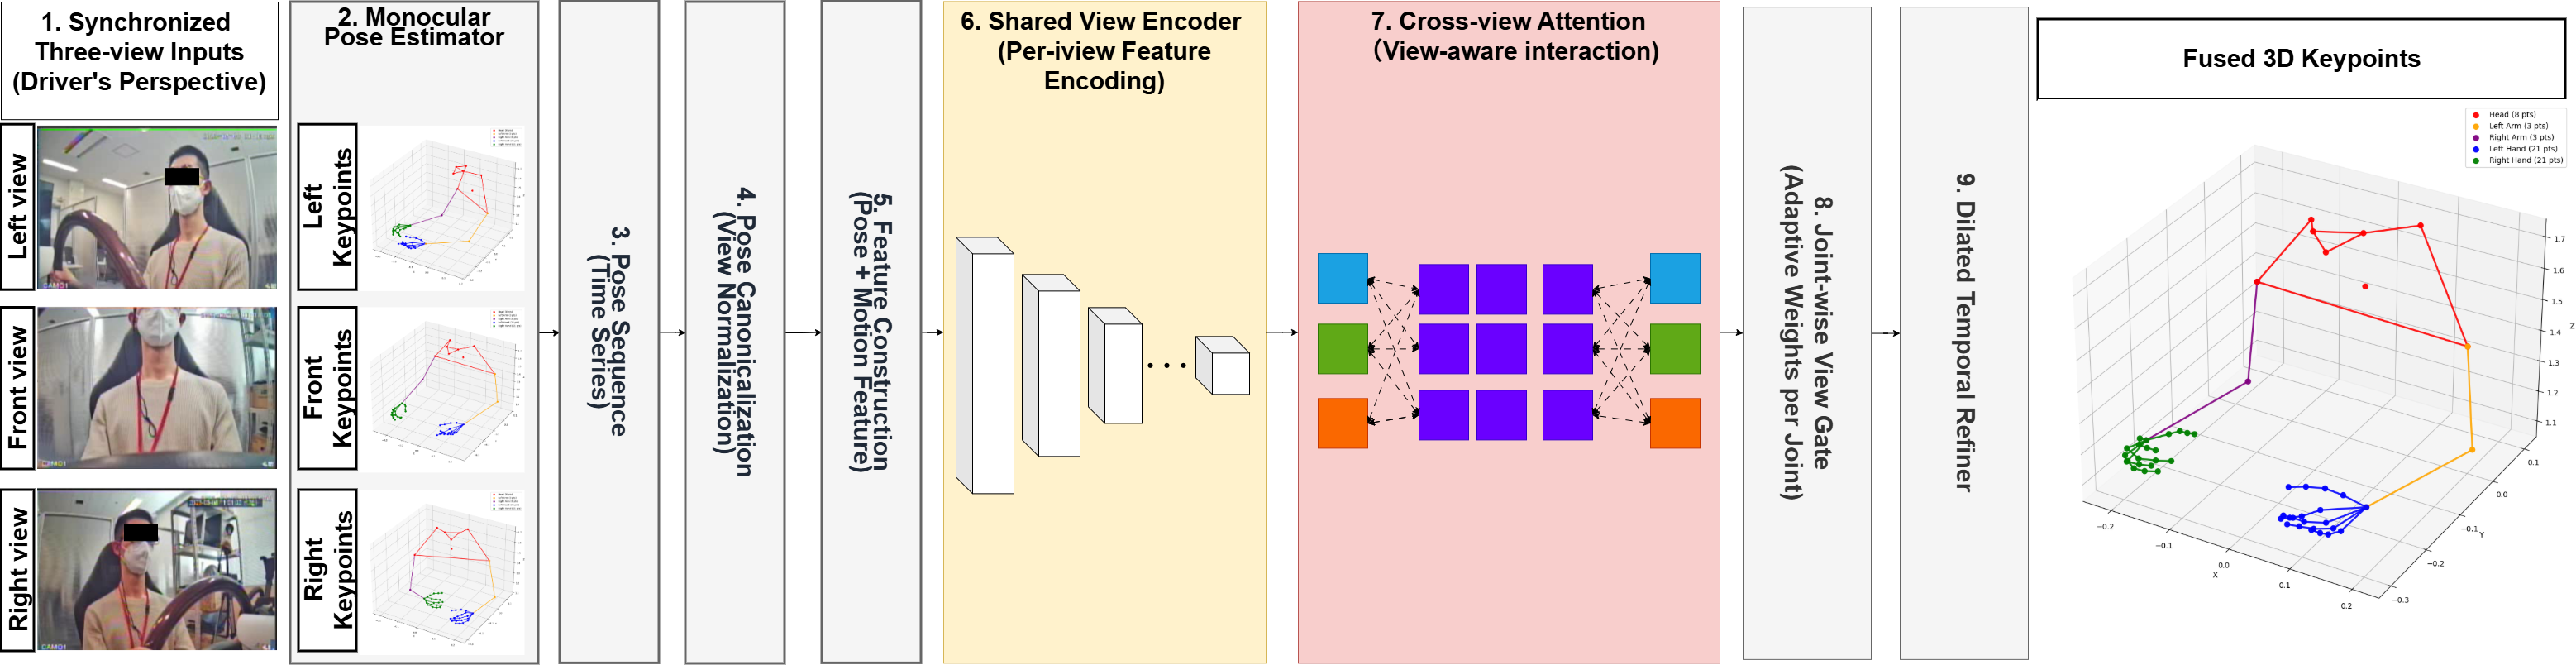
\includegraphics[width=0.98\linewidth]{figures/flow_chart.png}
\caption{Overview of TriPoseFusion. Synchronized front, left, and right driver-view images are first converted into monocular keypoint streams. The fusion network arranges these streams into temporal pose sequences, applies outlier-aware body-centered canonicalization, constructs motion-aware per-view features, encodes them with a shared view encoder, performs cross-view attention and joint-wise adaptive view gating, and finally applies a dilated temporal refiner to produce fused 3D keypoints.}
\label{fig:pipeline}
\end{figure}

\subsection{Body-Centered Pose Canonicalization}
Raw monocular 3D keypoints can differ in translation, orientation, and scale across views. We canonicalize each pose into a body-centered frame before fusion. Let $o_t$ be the neck joint, and let the shoulder vector define the body horizontal axis. For each frame, we estimate a rotation $R_t$ from the neck, left shoulder, and right shoulder, and transform each view by
\begin{equation}
\bar{P}_{v}^{t,j}=R_t\left(P_{v}^{t,j}-o_t\right).
\label{equ:canon}
\end{equation}
This step removes global translation and aligns all views to a comparable body coordinate system. In the reported 52-keypoint layout, the neck index is 51 and the left/right shoulder indices are 5 and 6. The robust variant first computes the shoulder distance $d_t=\|s^r_t-s^l_t\|_2$. A frame is treated as unreliable when $d_t<\epsilon$ or $d_t>2d_0$, where $\epsilon=10^{-6}$ and the shoulder-width prior is $d_0=0.5$ m. In reliable frames, the $x$ axis is the normalized shoulder direction, the downward axis is the shoulder midpoint minus the neck (or the mid-hip vector when available), and the final orthonormal frame is formed by cross products. In unreliable frames, both shoulder anchors are replaced by the neck before axis construction, yielding a neck-centered fallback frame rather than an arbitrary shoulder-derived rotation. The down-axis norm is clipped to $[\epsilon,1.0]$ and all axes are normalized with $\epsilon$ for numerical stability. The canonicalized pose sequence is then used as the input to the feature-construction stage described below.

\subsection{Multi-Scale Motion-Aware View Encoding}
For each view, frame, and joint, we construct a 3D motion-aware feature vector from the canonicalized pose stream:
\begin{equation}
\phi_{v}^{t,j}=\left[\bar{P}_{v}^{t,j};\dot{P}_{v,1}^{t,j};\dot{P}_{v,3}^{t,j};\dot{P}_{v,5}^{t,j};\ddot{P}_{v}^{t,j};\dddot{P}_{v}^{t,j}\right],
\end{equation}
where $\dot{P}_{v,k}^{t,j}$ denotes the finite difference $\bar{P}_{v}^{t,j}-\bar{P}_{v}^{t-k,j}$, and $\ddot{P}$ and $\dddot{P}$ denote first differences of velocity and acceleration. Boundary frames use the nearest available previous frame. Thus the reported model uses only canonicalized 3D positions, 3D velocities at strides 1, 3, and 5, and higher-order acceleration/jerk cues as input features. A shared MLP encoder maps these features into latent tokens:
\begin{equation}
H_{v}^{t,j}=\mathrm{MLP}(\phi_{v}^{t,j}).
\label{equ:encoder}
\end{equation}
Figure~\ref{fig:feature_construction} illustrates the core construction process for one canonicalized view sequence. Each joint token combines its current 3D coordinate with single-frame velocity, multi-scale velocity over 3- and 5-frame neighborhoods, and higher-order acceleration/jerk cues, producing a per-view tensor of shape $T\times J\times d$. The encoder consists of layer normalization, a linear projection to hidden dimension 128, GELU activation, dropout, a second linear layer, and GELU activation. This shared encoder exposes both instantaneous pose and temporal dynamics to the fusion module without introducing view-specific parameters before attention.

\begin{figure}[t]
\centering
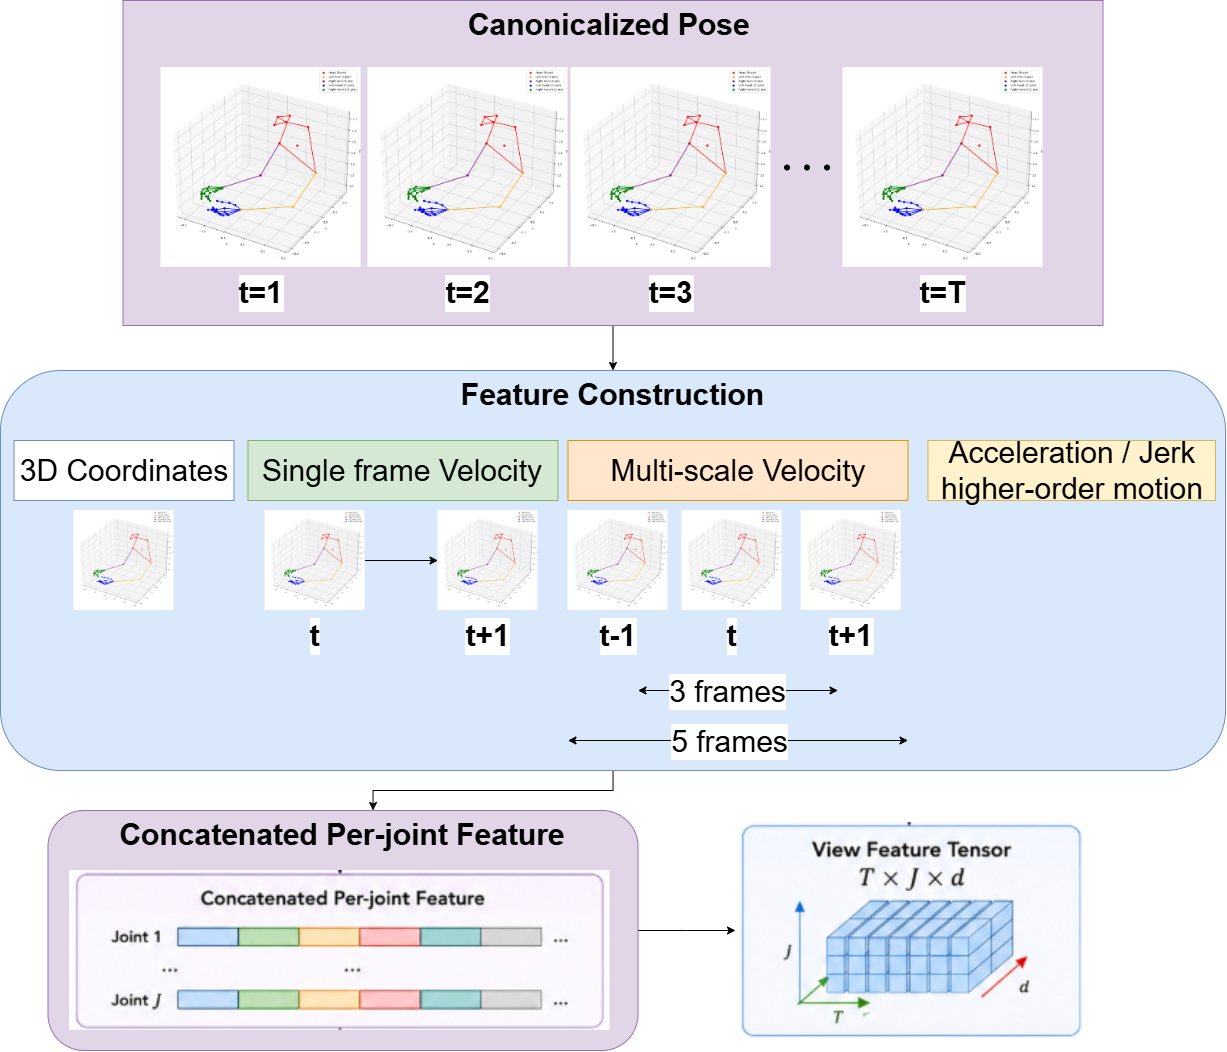
\includegraphics[width=0.75\linewidth]{figures/feature_construction.png}
\caption{Motion-aware feature construction from a canonicalized pose sequence. For each view, the model concatenates per-joint 3D coordinates with single-frame velocity, multi-scale velocity, and acceleration/jerk cues to form a $T\times J\times d$ view feature tensor before shared encoding.}
\label{fig:feature_construction}
\end{figure}

\subsection{Cross-View Attention with View Embeddings}
After shared encoding, TriPoseFusion performs attention only along the view dimension. For a fixed frame $t$ and joint $j$, the front, left, and right features form a short token set. We add a learnable view embedding to each token so that the attention module can distinguish camera identity after the shared encoder:
\begin{equation}
Z_{v}^{t,j}=H_{v}^{t,j}+e_{v}^{\mathrm{view}},\quad
\tilde{H}^{t,j}=\mathrm{MHSA}\left([Z_{1}^{t,j},\dots,Z_{V}^{t,j}]\right).
\label{equ:viewattn}
\end{equation}
The operation is local in time and joint index: it compares only the views of the same joint at the same timestamp, rather than attending across all frames or all joints. In implementation, the encoded tensor is reshaped from $(B,T,J,V,H)$ to $(BTJ,V,H)$ and processed with batch-first multi-head attention, then reshaped back to $(B,T,J,V,H)$. Because $V=3$, this module adds little computational overhead while allowing each view token to incorporate complementary evidence from the other cameras before view gating.

\subsection{Joint-Wise Adaptive View Gating}
Instead of predicting a single frame-level weight, TriPoseFusion estimates joint-wise and time-varying view reliability:
\begin{equation}
\alpha_{t,j,v}=\mathrm{softmax}_{v}\left(g(\tilde{H}_{v}^{t,j})\right),\quad
P_{\mathrm{init}}^{t,j}=\sum_{v=1}^{V}\alpha_{t,j,v}\bar{P}_{v}^{t,j}.
\label{equ:gating}
\end{equation}
The gate function $g(\cdot)$ is implemented as layer normalization, a linear layer from 128 to 64 channels, GELU activation, and a final linear projection to one logit per view. A softmax over the view dimension produces $\alpha_{t,j,v}$. The gate is included because different joints can be occluded in different cameras, but in the reported run its entropy regularization keeps the average weights close to uniform; we therefore interpret the gate as a stable learned fusion layer rather than as the main source of the observed gain.

\subsection{Dilated Temporal Pose Refinement}
The initial fused pose can still contain jitter from noisy keypoints. We therefore use a dilated temporal convolution network to predict a residual correction:
\begin{equation}
P_{\mathrm{final}}=P_{\mathrm{init}}+\Delta P,\quad
\Delta P=\mathrm{TCN}_{\mathrm{dilated}}(P_{\mathrm{init}}).
\label{equ:tcn}
\end{equation}
The refiner reshapes $P_{\mathrm{init}}$ to a $(B,3J,T)$ sequence and applies four 1D convolution blocks with kernel size 3, batch normalization, GELU, dropout, and dilation factors 1, 2, 4, and 8. A final $1\times1$ convolution maps the hidden sequence back to $3J$ residual channels. Its weights and biases are initialized to zero, so the model begins from the gated fused pose and learns only corrective residuals. Dilated convolutions enlarge the temporal receptive field to cover the 16-frame clip efficiently, enabling the model to handle slow motion and suppress high-frequency jitter.

\subsection{Training Objective}
The total self-supervised objective is
\begin{equation}
\mathcal{L}=\lambda_{tri}\mathcal{L}_{tri}+\lambda_{view}\mathcal{L}_{view}+\lambda_{bone}\mathcal{L}_{bone}+\lambda_{temp}\mathcal{L}_{temp}+\lambda_{nce}\mathcal{L}_{nce}+\lambda_{gate}\mathcal{L}_{gate}.
\label{equ:loss}
\end{equation}
$\mathcal{L}_{tri}$ is a Smooth L1 teacher loss. When a triangulated teacher is provided during training, it is canonicalized and used directly. In the reported experiments, no manually corrected triangulated 3D reference is used as training supervision; instead, the median of the canonicalized multi-view input poses is used as a robust pseudo teacher. $\mathcal{L}_{view}$ keeps the fused pose close to the canonicalized per-view observations, weighted by the detached gate weights. $\mathcal{L}_{bone}$ regularizes the left-right shoulder, neck-left shoulder, and neck-right shoulder lengths against the pre-refinement fused pose. $\mathcal{L}_{temp}$ penalizes acceleration magnitude to suppress temporal jitter. $\mathcal{L}_{nce}$ projects hidden view tokens to a 64-dimensional space and applies bidirectional InfoNCE between synchronized view pairs. Finally, $\mathcal{L}_{gate}=\log V + \sum_{v}\alpha_{t,j,v}\log\alpha_{t,j,v}$ encourages high-entropy view usage and prevents early collapse to a single camera.

\subsection{Implementation Details}
The reported model uses three input views (front, left, and right), 52 body keypoints, outlier-aware canonicalization, and uniformly sampled 16-frame clips. The shared view encoder has hidden dimension 128 and is applied independently to each view before cross-view attention. Cross-view attention uses four heads with learnable view embeddings. The temporal refiner is a four-layer dilated TCN with hidden dimension 256, kernel size 3, dilation factors 1, 2, 4, and 8, and a residual output initialized to zero. Dropout is set to 0.1.

Training uses AdamW with learning rate $10^{-4}$, weight decay $10^{-5}$, batch size 30 per GPU, two GPUs, gradient clipping at 1.0, and a maximum of 50 epochs. The loss weights are $\lambda_{tri}=1.0$, $\lambda_{view}=0.2$, $\lambda_{bone}=0.5$, $\lambda_{temp}=0.1$, $\lambda_{nce}=0.1$, and $\lambda_{gate}=0.01$. The manually corrected triangulated pseudo ground truth is reserved for evaluation and is not used by the reported training run.

%===========================================================
\section{Experiments}
\label{sec:experiments}

\subsection{Dataset}
We evaluate on a synchronized tri-view in-cabin driver monitoring dataset collected in a driving-simulator environment. Each driving sequence is recorded from three fixed camera views: front, left, and right. The camera layout is designed to provide complementary observations of the driver: the front view captures frontal upper-body motion and head pose, while the two side views provide additional evidence for arms, shoulders, and hands when the steering wheel or self-occlusion degrades the frontal observation. Figure~\ref{fig:dataset_examples} shows the simulator setup, camera arrangement, and representative daytime and nighttime frames.

\begin{figure}[t]
\centering
\begin{minipage}[t]{0.235\linewidth}
\centering
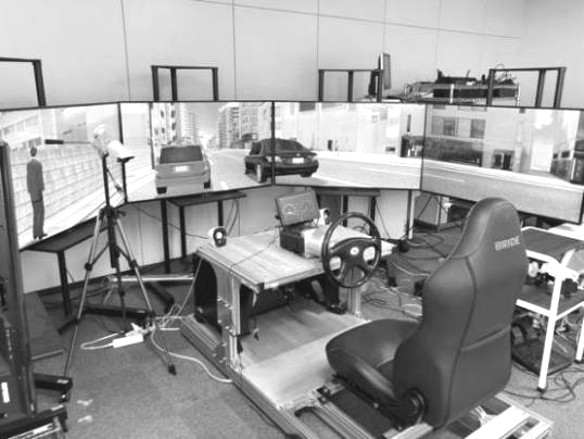
\includegraphics[width=\linewidth]{figures/dataset/driving_simulator.jpg}\\[-1mm]
{\scriptsize (a) Simulator}
\end{minipage}
\hfill
\begin{minipage}[t]{0.235\linewidth}
\centering
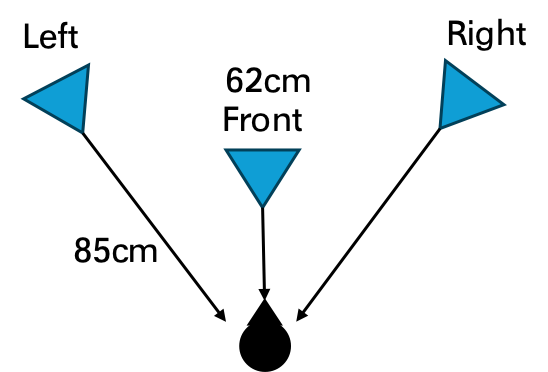
\includegraphics[width=\linewidth]{figures/dataset/camera_config.png}\\[-1mm]
{\scriptsize (b) Cameras}
\end{minipage}
\hfill
\begin{minipage}[t]{0.235\linewidth}
\centering
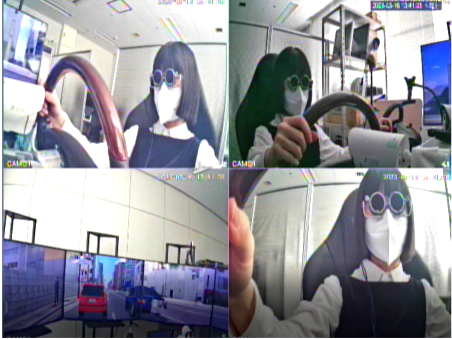
\includegraphics[width=\linewidth]{figures/dataset/day.png}\\[-1mm]
{\scriptsize (c) Daytime}
\end{minipage}
\hfill
\begin{minipage}[t]{0.235\linewidth}
\centering
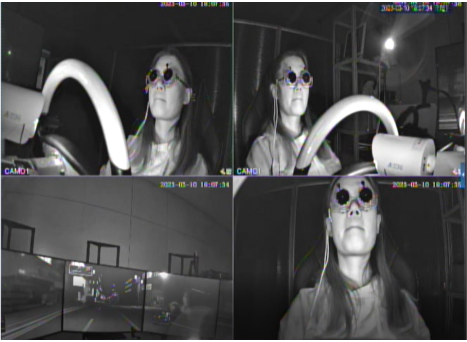
\includegraphics[width=\linewidth]{figures/dataset/night.png}\\[-1mm]
{\scriptsize (d) Nighttime}
\end{minipage}
\caption{Dataset acquisition setting and visual examples. The simulator provides a controlled in-cabin driving scene, while the fixed tri-view camera layout records complementary observations of the seated driver. The daytime and nighttime examples illustrate the illumination variation, steering-wheel occlusion, and view-dependent visibility changes that motivate robust multi-view keypoint fusion.}
\label{fig:dataset_examples}
\end{figure}

The four panels in Figure~\ref{fig:dataset_examples} show the simulator platform, fixed tri-view camera configuration, and representative daytime and nighttime frames. The examples highlight the main visual challenges: steering-wheel occlusion, view-dependent visibility of arms and hands, screen reflections in daytime capture, and low-brightness or high-contrast regions at night.

The dataset contains four illumination/environment settings: day-high, day-low, night-high, and night-low. These settings correspond to daytime or nighttime capture under high- or low-activity illumination conditions. The reported comparison covers 22 subjects and 88 matched subject-environment sequences, with one sequence per subject in each illumination setting. This balanced evaluation allows us to test whether fusion remains useful across both daytime and nighttime driving conditions. The complete dataset composition used in the reported comparison is listed in Table~\ref{tab:dataset_stats}.

For each camera view, an off-the-shelf monocular pose estimator produces per-frame SAM3D body outputs saved as \texttt{.npz} files. We use the synchronized front/left/right 3D keypoint streams as the input to TriPoseFusion; RGB frames are shown in Figure~\ref{fig:dataset_examples} only to document the capture setting and are not used by the fusion model. To focus on driver-monitoring-relevant body parts, we keep a 52-keypoint subset consisting of head keypoints, shoulder/neck landmarks, and hand keypoints. A sample is considered valid only when all requested views are available, which ensures that the fusion model always receives temporally aligned multi-view evidence for the same driver motion.

\begin{table}[t]
\centering
\caption{Dataset composition used in the reported comparison. Each subject contributes one sequence per illumination setting.}
\label{tab:dataset_stats}
\scriptsize
\setlength{\tabcolsep}{4pt}
\begin{tabular}{lcccc}
\hline
Setting & Internal label & Subjects & Sequences & Views / Keypoints \\
\hline
Day high & day\_high & 22 & 22 & 3 / 52 \\
Day low & day\_low & 22 & 22 & 3 / 52 \\
Night high & night\_high & 22 & 22 & 3 / 52 \\
Night low & night\_low & 22 & 22 & 3 / 52 \\
\hline
Total & -- & 22 & 88 & 3 / 52 \\
\hline
\end{tabular}
\end{table}

\subsection{Evaluation Protocol}
The dataloader builds temporal chunks from each subject-environment sequence by using the minimum available frame count across the three views, so all views remain synchronized. Each chunk is uniformly sampled to 16 frames for model input and evaluation. Training and evaluation use subject-disjoint GroupKFold partitions generated from person identifiers, so sequences from the same driver do not appear in both training and validation for a given fold. The reported main comparisons use the same validation fold and the same matched subject-environment pairs for all methods in the corresponding table. The evaluation compares TriPoseFusion with front-only, left-only, right-only, best-single-view, and fixed-rule multi-view baselines. The best-single-view baseline is an oracle sequence-level baseline: for each subject-environment sequence, we report the lowest-error single camera under the evaluation reference. It is included as a strong diagnostic reference rather than as a deployable camera-selection method.

\subsection{Pseudo Ground Truth}
The geometric reference is constructed from synchronized multi-view 2D keypoints that are manually checked and corrected before triangulation. The pipeline is: (1) load synchronized front/left/right 2D keypoint annotations, (2) correct missing or inaccurate joints by human inspection, (3) align the streams by frame ID, (4) triangulate the corrected multi-view 2D keypoints to obtain a 3D reference, and (5) save both 3D keypoints and a valid-joint mask for evaluation. During evaluation, frame IDs from the source SAM3D sequence are matched strictly to frame IDs in the triangulated reference, so predictions and pseudo ground truth are compared at the same timestamps. Metrics are computed only over valid joints. Since this reference is triangulated from manually corrected 2D keypoints rather than captured by a motion-capture system, we refer to it as pseudo ground truth. The reported numbers therefore measure agreement with this corrected triangulation reference and should not be interpreted as absolute mocap accuracy. This protocol is nevertheless useful for testing whether tri-view fusion produces poses that are more geometrically consistent than any individual monocular view.

Manual correction is used only to construct the evaluation reference in the reported experiments. It is not provided to the fusion model as a training target.

To characterize the quality of the triangulation reference itself, we also report its multi-view reprojection error in Table~\ref{tab:triangulation_quality}. The statistics are computed over the same 88 subject-environment sequences and the same 52-keypoint subset used for model evaluation, after filtering by the triangulation valid-joint mask. The mean reprojection error is 10.28 px and the median is 8.37 px over 17.15M valid triangulated joints. The 95th percentile is 26.02 px for the mean multi-view error, below the 40 px outlier-rejection threshold used during triangulation. Per-view errors are additionally reported to show the residual camera-specific projection mismatch. These values indicate that the pseudo ground truth is a useful corrected multi-view geometric reference, while still retaining non-negligible residual 2D localization, calibration, and synchronization noise.

\begin{table}[t]
\centering
\caption{Triangulation-reference quality for the pseudo ground truth used in evaluation. Reprojection errors are measured in pixels on the valid 52-keypoint evaluation subset. Environment rows report mean multi-view reprojection error; view rows report the corresponding per-view reprojection error, so their percentiles can exceed the mean-error filtering threshold.}
\label{tab:triangulation_quality}
\scriptsize
\setlength{\tabcolsep}{3pt}
\begin{tabular}{llccccc}
\hline
Group & Subset & Valid joints & Mean (px) & Median (px) & P90 (px) & P95 (px) \\
\hline
Overall & All & 17.15M & 10.28 & 8.37 & 21.88 & 26.02 \\
\hline
Environment & Day high & 4.37M & 10.19 & 8.25 & 22.11 & 26.31 \\
Environment & Day low & 4.19M & 10.18 & 8.29 & 22.12 & 26.53 \\
Environment & Night high & 4.61M & 10.73 & 8.99 & 21.71 & 25.26 \\
Environment & Night low & 3.98M & 9.96 & 7.98 & 21.66 & 26.11 \\
\hline
View & Front & 1.40M & 15.46 & 11.51 & 35.92 & 42.03 \\
View & Left & 16.88M & 9.96 & 8.29 & 20.81 & 24.58 \\
View & Right & 16.02M & 10.16 & 8.18 & 21.84 & 26.31 \\
\hline
\end{tabular}
\end{table}

\subsection{Evaluation Metrics}
We report standard 3D pose metrics: MPJPE (mean per-joint position error), PA-MPJPE after Procrustes alignment, and PCK under distance thresholds. Unless otherwise specified, all 3D distance errors in the experimental tables are reported in meters. Before MPJPE computation, predictions and the triangulated reference are compared in the common 52-keypoint model space after positive scale alignment and body-anchor translation alignment, using the same alignment protocol for all methods and without applying a rotation. PA-MPJPE additionally applies a per-sample Procrustes similarity transform, so it highlights residual pose-shape quality after removing global translation, rotation, and scale differences. We report PCK@0.10, which counts a joint as correct if its 3D error is below 0.10 m after the MPJPE alignment. This threshold is strict for the noisy upper-body and hand-focused pseudo-reference used here, so PCK is treated as a secondary diagnostic metric and should be interpreted together with MPJPE and PA-MPJPE rather than as an isolated accuracy measure.

\subsection{Baselines}
We compare TriPoseFusion with single-view baselines (front/left/right) and the best single-view result for each subject-environment pair. These baselines isolate whether adaptive tri-view fusion improves over selecting the strongest individual camera. We report the best single view as an oracle single-camera baseline because it assumes access to the strongest camera for each sequence. We also evaluate fixed-rule multi-view fusion baselines, including arithmetic mean and coordinate-wise median. These rule-based baselines test whether the improvement comes simply from using multiple cameras or from geometry-normalized learned fusion. To separate learned fusion from pose normalization, we additionally report a diagnostic canonicalized-baseline matrix in which the same body-centered canonicalization is applied to the input keypoint streams before non-learned single-view, fixed-fusion, and temporal-smoothing operations are evaluated.

We do not report external benchmark accuracies because published image- or heatmap-based multi-view pose estimators assume different inputs, keypoint definitions, supervision, and evaluation references. The quantitative comparisons below therefore focus on baselines that can be evaluated under the same keypoint-level protocol. Stronger image-level baselines, such as learnable triangulation or volumetric fusion variants, remain important future comparisons once matched image features, calibration, and valid-frame coverage are available for the same split.

\subsection{Main Comparison}
\begin{table}[t]
\centering
\caption{Main pose fusion comparison over 88 matched subject-environment sequences. Raw single-view rows evaluate the original monocular predictions, while canonicalized rows apply the same body-centered normalization before fixed-rule fusion. Lower MPJPE/PA-MPJPE and higher PCK are better. Metrics are measured against pseudo ground truth in meters.}
\label{tab:main_pose}
\scriptsize
\setlength{\tabcolsep}{2.5pt}
\begin{tabular}{lccc}
\hline
Method & MPJPE (m) $\downarrow$ & PA-MPJPE (m) $\downarrow$ & PCK@0.10 $\uparrow$ \\
\hline
\multicolumn{4}{l}{\emph{Raw single-view baselines}} \\
Front only & 2.140 & 1.316 & 0.000 \\
Left only & 2.090 & 1.489 & 0.000 \\
Right only & 2.093 & 1.412 & 0.000 \\
Best single & 2.078 & 1.275 & 0.000 \\
\hline
\multicolumn{4}{l}{\emph{Canonicalized non-learned baselines}} \\
Front single, canonicalized & 0.969 & 1.664 & 0.116 \\
Left single, canonicalized & 0.929 & 1.516 & 0.110 \\
Right single, canonicalized & 0.954 & 1.606 & 0.107 \\
Best canonicalized single & 0.927 & 1.504 & 0.113 \\
Mean fusion, canonicalized & 0.948 & 1.594 & 0.111 \\
Median fusion, canonicalized & 0.946 & 1.589 & 0.112 \\
Median fusion + smoothing & 0.947 & 1.590 & 0.112 \\
\hline
\multicolumn{4}{l}{\emph{Learned fusion}} \\
TriPoseFusion & \textbf{0.412} & \textbf{0.275} & \textbf{0.141} \\
\hline
\end{tabular}
\end{table}

Table~\ref{tab:main_pose} shows that TriPoseFusion consistently improves agreement with the corrected triangulation reference. Compared with the best available raw single camera for each sequence, MPJPE decreases by 1.666 m, an 80.2\% relative reduction. The large raw single-view errors reflect keypoint-stream mismatch under inconsistent monocular 3D frames rather than pure local pose-shape error. PCK@0.10 increases from 0.000 to 0.141, although this threshold remains strict for the upper-body and hand-focused pseudo-reference. PA-MPJPE improves by 1.000 m on average, with TriPoseFusion outperforming the best single view on 47 of 88 sequences.

The canonicalized non-learned baselines show that normalization and naive use of all three views are not sufficient by themselves. The best canonicalized single view still has 0.927 m MPJPE, and mean, median, and smoothed median fusion remain far from TriPoseFusion. The gains are also stable across illumination: relative to the canonicalized best-single baseline, day-high, day-low, night-high, and night-low MPJPE reductions are 0.371, 0.742, 0.415, and 0.519 m. Figure~\ref{fig:qualitative_pose} provides qualitative examples in the same 52-keypoint model space, illustrating that the fused predictions better follow the corrected multi-view reference under upper-body and hand ambiguity.

\begin{figure}[t]
\centering
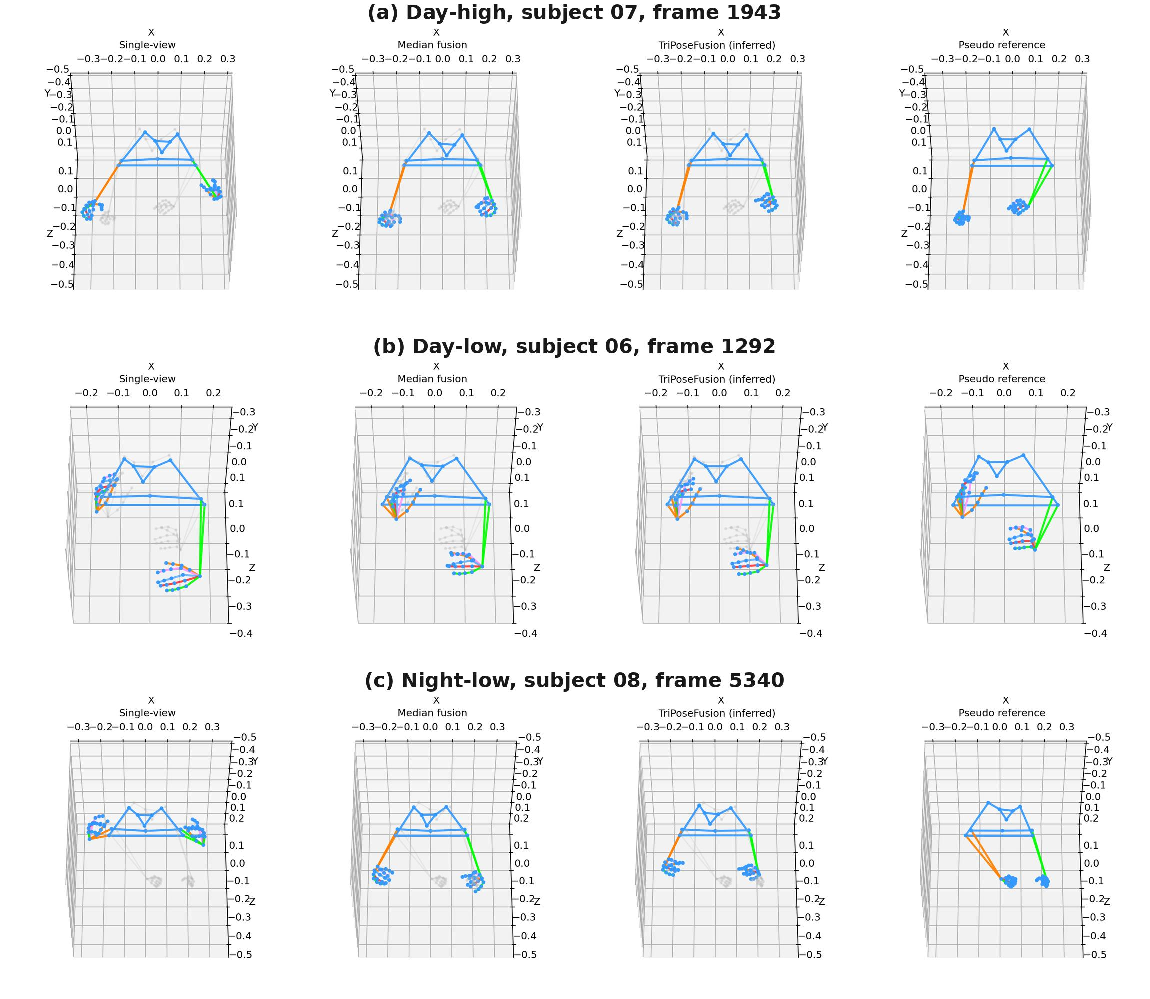
\includegraphics[width=0.82\linewidth]{figures/fig_qualitative_pose.pdf}
\caption{Qualitative pose examples in the common 52-keypoint model space. The visualization compares TriPoseFusion predictions with the corrected triangulation reference after the same scale and body-anchor alignment used for diagnostic rendering.}
\label{fig:qualitative_pose}
\end{figure}

\subsection{Component Ablation}
\begin{table}[t]
\centering
\caption{Component ablation under the matched three-view evaluation setting. MPJPE and PA-MPJPE are reported in meters. The largest change comes from robust body-centered canonicalization; other modules provide smaller secondary effects in this run.}
\label{tab:ablation}
\scriptsize
\setlength{\tabcolsep}{4pt}
\begin{tabular}{lccc}
\hline
Configuration & MPJPE (m) $\downarrow$ & PA-MPJPE (m) $\downarrow$ & PCK@0.10 $\uparrow$ \\
\hline
Base & 0.846 & 0.857 & 0.140 \\
Base + dilated TCN & 0.845 & 0.855 & 0.140 \\
Base + multi-scale velocity & 0.845 & 0.855 & 0.141 \\
Base + gate entropy & 0.846 & 0.857 & 0.140 \\
Base + robust canonicalization & 0.412 & 0.274 & 0.139 \\
Full TriPoseFusion & 0.412 & 0.275 & \textbf{0.141} \\
\hline
\end{tabular}
\end{table}

The ablation in Table~\ref{tab:ablation} indicates that robust pose canonicalization is the dominant contributor in this setting. The base model obtains 0.846 m MPJPE, while adding robust canonicalization reduces MPJPE to 0.412 m, a 51.3\% relative reduction. In contrast, adding dilated temporal convolution, multi-scale velocity features, or gate entropy alone changes MPJPE only marginally. The full model preserves the canonicalization gain but does not further reduce MPJPE in this run, suggesting that the largest error source is cross-view coordinate-frame and outlier mismatch rather than temporal jitter alone. Additional diagnostic gating and attention ablations are reported in the supplementary material. The learned gate remains close to uniform, with mean front/left/right weights of 0.33334/0.33334/0.33335, indicating non-collapse but not strong adaptive view selection.

\subsection{Discussion and Limitations}
TriPoseFusion still depends on the upstream pose estimator. The fixed-rule fusion and ablation results show that most of the current gain comes from robust body-centered canonicalization, while temporal and gating modules provide smaller secondary effects under the pseudo-ground-truth protocol. Several limitations remain: the evaluation reference is manually corrected triangulation rather than mocap, so metrics measure corrected multi-view geometric consistency; the comparison is restricted to keypoint-level baselines and does not yet include raw 2D triangulation, learnable triangulation, or volumetric image-feature fusion under the same split; the dataset is a controlled simulator with fixed cameras; and failures remain likely when all views miss the same body part or when the pseudo ground truth contains residual 2D, calibration, synchronization, or triangulation error.

%===========================================================
\section{Conclusion}
TriPoseFusion shows that robust geometry normalization can make noisy multi-view driver keypoints substantially more consistent with a corrected triangulation reference. On 88 matched subject-environment sequences, the 80.2\% MPJPE reduction over an oracle best-single-view baseline is driven primarily by outlier-aware body-centered canonicalization, with lightweight fusion and temporal refinement serving as compact supporting modules.

%===========================================================
\bibliographystyle{splncs}
\bibliography{egbib}

\end{document}
